\documentclass[nooutcomes]{ximera}
%\documentclass[space,handout,nooutcomes]{ximera}

% For preamble materials

\usepackage{pgf,tikz}
\usepackage{mathrsfs}
\usetikzlibrary{arrows}
\usepackage{framed}
\usepackage{amsmath}
\pgfplotsset{compat=1.17}

\def\fixnote#1{\begin{framed}{\textcolor{red}{Fix note: #1}}\end{framed}}  % Allows insertion of red notes about needed edits
%\def\fixnote#1{}

\def\detail#1{{\textcolor{blue}{Detail: #1}}}   

\pdfOnly{\renewenvironment{image}[1][]{\begin{center}}{\end{center}}}

\graphicspath{
  {./}
  {chapter1/}
  {chapter2/}
  {chapter4/}
  {proofs/}
  {graphics/}
  {../graphics/}
}

\newenvironment{sectionOutcomes}{}{}


%%% This set of code is all of our user defined commands
\newcommand{\bysame}{\mbox{\rule{3em}{.4pt}}\,}
\newcommand{\N}{\mathbb N}
\newcommand{\C}{\mathbb C}
\newcommand{\W}{\mathbb W}
\newcommand{\Z}{\mathbb Z}
\newcommand{\Q}{\mathbb Q}
\newcommand{\R}{\mathbb R}
\newcommand{\A}{\mathbb A}
\newcommand{\D}{\mathcal D}
\newcommand{\F}{\mathcal F}
\newcommand{\ph}{\varphi}
\newcommand{\ep}{\varepsilon}
\newcommand{\aph}{\alpha}
\newcommand{\QM}{\begin{center}{\huge\textbf{?}}\end{center}}

\renewcommand{\le}{\leqslant}
\renewcommand{\ge}{\geqslant}
\renewcommand{\a}{\wedge}
\renewcommand{\v}{\vee}
\renewcommand{\l}{\ell}
\newcommand{\mat}{\mathsf}
\renewcommand{\vec}{\mathbf}
\renewcommand{\subset}{\subseteq}
\renewcommand{\supset}{\supseteq}
%\renewcommand{\emptyset}{\varnothing}
%\newcommand{\xto}{\xrightarrow}
%\renewcommand{\qedsymbol}{$\blacksquare$}
%\newcommand{\bibname}{References and Further Reading}
%\renewcommand{\bar}{\protect\overline}
%\renewcommand{\hat}{\protect\widehat}
%\renewcommand{\tilde}{\widetilde}
%\newcommand{\tri}{\triangle}
%\newcommand{\minipad}{\vspace{1ex}}
%\newcommand{\leftexp}[2]{{\vphantom{#2}}^{#1}{#2}}

%% More user defined commands
\renewcommand{\epsilon}{\varepsilon}
\renewcommand{\theta}{\vartheta} %% only for kmath
\renewcommand{\l}{\ell}
\renewcommand{\d}{\, d}
\newcommand{\ddx}{\frac{d}{dx}}
\newcommand{\dydx}{\frac{dy}{dx}}


\usepackage{bigstrut}


%\usepackage{tikz}


\title{Symmetry}
\author{Bart Snapp and Brad Findell}
\begin{document}
\begin{abstract}
Short-answer questions about symmetry. 
\end{abstract}
\maketitle

\begin{question}
Categorize the capital letters of the alphabet by their symmetries.  Use the following font: 
\begin{image}
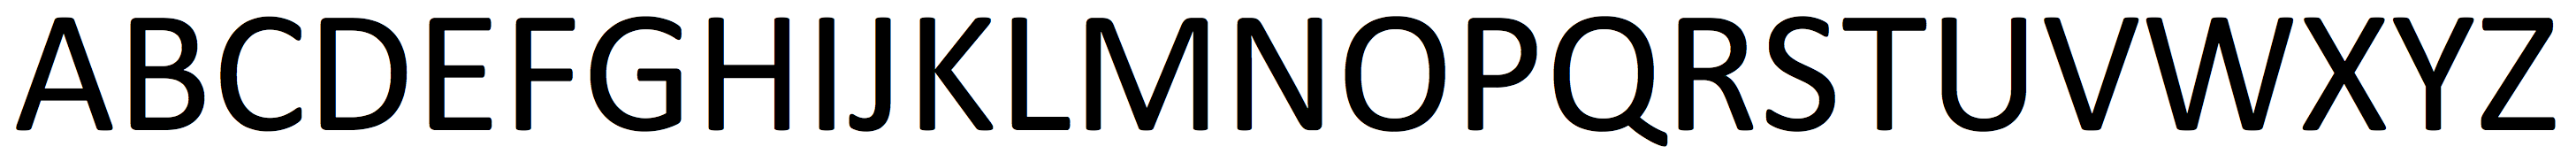
\includegraphics{alphabet.png}
\end{image}
%\begin{tikzpicture}
%  \node {\scalebox{10}{\textsf{K}}};
%\end{tikzpicture}
\begin{itemize}
\item Vertical line symmetry:  $\answer{AHIMOTUVWXY}$
\item Horizontal line symmetry:  $\answer{BCDEHIKOX}$  
\item $180^\circ$ rotational symmetry: $\answer{HINOSXZ}$
\item None: $\answer{FGJLPQR}$
\end{itemize}
\begin{feedback}[correct]
Notes:  (1) In many fonts that look much the same, B and K have no symmetry.  (2) In this font, the O is slightly taller than it is wide.  If it were a circle, there would be more symmetry.  (See later problem.)
\end{feedback}
\end{question}

\begin{question}
Write the words COKE and PEPSI in capital letters so that they read vertically.  Use a mirror to look at a reflection of the words.  What is different about the reflections of the two words?  Explain.  
\begin{freeResponse}
\end{freeResponse}
\begin{hint}
If the K has horizontal line symmetry in the font, then all the letters in COKE have horizontal line symmetry, which becomes vertical line symmetry when the word is written vertically. PEPSI, on the other hand, has several letters without that symmetry.  
\end{hint}
\end{question}


\begin{question}
We often say a figure is ``symmetric'' when we notice that it has symmetry, but now we want to be more precise:  

A \emph{symmetry} of a figure is a
\wordChoice{\choice{reflection}\choice{rotation}\choice[correct]{transformation}\choice{translation}} 
that maps a figure 
\wordChoice{\choice{to its opposite}\choice[correct]{onto itself}\choice{to another figure}}.  
\end{question}

\begin{question}
Explain why a sequence of two symmetries of a figure must also be a symmetry of that figure.  
\begin{freeResponse}
\end{freeResponse}
\begin{hint}
%If a transformation T1 maps a figure onto itself and another transformation T2 maps the figure onto itself, then T1 followed by T2 also maps the figure onto itself.  
The first transformation maps the figure onto itself, and the second transformation maps the figure onto itself, so the sequence of two transformations maps the figure $\answer[format=string]{onto itself}$.  
\end{hint}
\end{question}

\begin{question}
Explain why the identity transformation should be considered a symmetry of \emph{any} figure.   

\textbf{Some possible explanations:} 
\begin{itemize}
\item The identity transformation satisfies the definition of a symmetry: It maps the figure $\answer[format=string]{onto itself}$ (two words). 
\item If a figure has reflection symmetry $R_k$ about a line $k$, then $R_k$ followed by $R_k$ is the $\answer[format=string]{identity transformation}$ (two words).  And by the previous result, this sequence of symmetries must also be a symmetry.  
\item If a figure has rotational symmetry $R_\alpha$ by some angle $\alpha$ about some center, then it must also have a rotational symmetry $R_{-\alpha}$ by the angle $-\alpha$ about the same center.  $R_\alpha$ followed by $R_{-\alpha}$ is the $\answer[format=string]{identity transformation}$ (two words).  And by the previous result, this sequence of symmetries must also be a symmetry.  
\end{itemize}
\begin{feedback}[correct]
Note: Sometimes the identity transformation is called the \emph{trivial} symmetry.  If the identity transformation is the \emph{only} symmetry of a figure, we usually say the figure is asymmetric or has no (nontrivial) symmetry.  
\end{feedback}
\end{question}

\begin{question}
It is reasonable to call the identity transformation a translation because it is a translation of magnitude $\answer{0}$ in any direction.  

It is reasonable to call the identity transformation a rotation because it is a rotation of $\answer{0}$ degrees about any center.  
\end{question}

\begin{question}
Indicate the number of rotation and reflection symmetries of the following figures (including the identity rotation): 
\begin{enumerate}
\item An equilateral triangle: $\answer{3}$ rotation(s) and $\answer{3}$ reflection(s). 
\item An isosceles triangle that is not equilateral: $\answer{0}$ rotation(s) and $\answer{1}$ reflection(s).
\item A square: $\answer{4}$ rotation(s) and $\answer{4}$ reflection(s).
\item A rectangle that is not a square: $\answer{2}$ rotation(s) and $\answer{2}$ reflection(s).
\item A rhombus that is not a square: $\answer{2}$ rotation(s) and $\answer{2}$ reflection(s).
\item A (non-special) parallelogram: $\answer{2}$ rotation(s) and $\answer{0}$ reflection(s).
\item A regular $n-$gon: $\answer{n}$ rotation(s) and $\answer{n}$ reflection(s).
\end{enumerate}
\end{question}

%\begin{question}
%Describe all of the symmetries of the following figures: 
%\begin{enumerate}
%\item An equilateral triangle
%\item An isosceles triangle that is not equilateral
%\item A square
%\item A rectangle that is not a square
%\item A rhombus that is not a square
%\item A (non-special) parallelogram
%\item A regular $n$-gon
%\end{enumerate}
%\end{question}


\begin{question}
Suppose that quadrilateral $ABCD$ has exactly one rotation symmetry (other than the identity transformation) and no reflection symmetry.  What kind(s) of quadrilateral could it be?  Explain your reasoning.  
\begin{freeResponse}
\end{freeResponse}
\begin{hint}
If a rotation of $\alpha$ is a symmetry of a figure, then a rotation of $2\alpha$ must also be a symmetry.  Thus, for the quadrilateral to have only one (non-identity) rotation symmetry, it must be that $\alpha = \answer{180}$ degrees.  That rotation will swap opposite vertices, which implies that the center of rotation is the midpoint of each diagonal, so that the diagonals must $\answer[format=string]{bisect}$ each other.  Thus, quadrilateral $ABCD$ is a $\answer[format=string]{parallelogram}$ that is not any more special (or it would have additional symmetry).  
\end{hint}
\end{question}

\begin{question}
Suppose that quadrilateral $ABCD$ has exactly one reflection symmetry and no rotation symmetry (other than the identity transformation).  What kind(s) of quadrilateral could it be?  Explain your reasoning.  
\begin{freeResponse}
\end{freeResponse}
\begin{hint}
A parallelogram has $180^\circ$ rotational symmetry, so quadrilateral $ABCD$ cannot be a parallelogram, which also excludes the special cases: rhombus, rectangle, and square.  If the line of symmetry goes through two vertices, 
it must be a(n) $\answer[format=string]{kite}$ that is not a rhombus.  If the line of symmetry goes through two sides, it must be a(n) $\answer[format=string]{isosceles trapezoid}$ (two words).  
\end{hint}
\end{question}

\begin{question}
What are the symmetries of a circle? 
\begin{freeResponse}
\end{freeResponse}
\begin{hint}
A circle has rotational symmetry by any $\answer[format=string]{angle}$ about its center.  A circle has reflection symmetry about any $\answer[format=string]{line}$ through its center.  A circle does not have translation symmetry.  
\end{hint}
\end{question}

\begin{question}
How can you use the symmetries of a circle to determine whether a figure is indeed a circle?  
\begin{freeResponse}
\end{freeResponse}
\begin{hint}
Perform any of the symmetry transformations to be sure that the circle is actually mapped onto itself.  
\end{hint}
\end{question}

\begin{question}
What are the symmetries of a line?  
\begin{freeResponse}
\end{freeResponse}
\begin{hint}
\begin{enumerate}
\item A line has translation symmetry by a vector of any length \wordChoice{\choice[correct]{parallel}\choice{perpendicular}\choice{opposite}} to the line.   
\item A line has $\answer{180}$ degree rotational symmetry about any point on the line.  
\item A line has reflection symmetry about any \wordChoice{\choice{parallel}\choice[correct]{perpendicular}\choice{opposite}} to the line.  A line also has reflection symmetry about itself.  
\end{enumerate}
\end{hint}
\end{question}

%\begin{question}
%Given a line, describe a rotation symmetry and a reflection symmetry that have the same effect on the line.  How do the corresponding transformations differ in what they do to the surrounding space?  
%\begin{freeResponse}
%\end{freeResponse}
%\begin{hint}
%Given a point $P$ on the line $k$, let $j$ be the unique line through $P$ perpendicular to $k$.  A $180^\circ$ rotation about $P$ and a reflection about $j$ have the same effect on the line $k$, even though those transformations have different effects on the rest of the plane.  
%\end{hint}
%\end{question}

\begin{question}
How can you use the symmetries of a line to determine whether a figure is indeed a line? 
\begin{freeResponse}
\end{freeResponse}
\begin{hint}
Perform any of the symmetry transformations to be sure that the line is actually mapped onto itself.  
\end{hint}
\end{question}

%\begin{question}
%Find some tessellations.  For each tessellation, describe all of its symmetries.  
%\begin{freeResponse}
%\end{freeResponse}
%\begin{hint}
%\end{hint}
%\end{question}



\end{document}
